\documentclass[a4paper,12pt,twoside]{article}

%PACKAGES

\usepackage[T1]{fontenc}
\usepackage{lmodern}

\usepackage[utf8]{inputenc}
\usepackage[slovak]{babel}
\usepackage{comment}

\usepackage{array}

\usepackage{graphicx,amsmath,amssymb, amsthm, multicol}
\usepackage{pdfpages}

\usepackage[nottoc]{tocbibind}
\usepackage{mathrsfs}
\usepackage{psfrag}
\usepackage[small,bf]{caption}
\usepackage{ifthen}

\usepackage{xcolor}
\usepackage{listings}
\usepackage{enumitem}

\usepackage[toc,page]{appendix}

\usepackage{url}
\urlstyle{rm}
\renewcommand\UrlFont{\color{black}}

\usepackage{pgfplots}
\pgfplotsset{compat=1.16}

\usepackage{tikz}
\usetikzlibrary{positioning,chains,fit,shapes,calc}

% \renewcommand{\familydefault}{\rmdefault}

\newtheorem{defin}{Definícia}[section]
\newtheorem{theorem}[defin]{Veta}
\newtheorem{prop}[defin]{Tvrdenie}
\newtheorem{lema}[defin]{Lema}
\newtheorem{cor}[defin]{Dôsledok}
\newtheorem{hypoteza}{Hypotéza}[section]
\newtheoremstyle{comment}{}{}{}{}{}{:}{ }{#1}
\theoremstyle{comment}
\newtheorem{dokaz}{Dôkaz}[section]
\newtheorem{com}{\textit{Poznámka}}

\usepackage{hyperref}                                     
\hypersetup{%  http://www.tug.org/applications/hyperref/
bookmarksnumbered,
pdfstartview={FitH},
linkcolor=black,
citecolor=black,
colorlinks=true,
pdfpagemode={None},
plainpages=false
}%

%%\usepackage{fullpage}
%%\setlength{\topmargin}{-0.5cm}
%%\setlength{\headheight}{0cm}
%%\setlength{\headsep}{0in}
\setlength{\textheight}{24cm}
\setlength{\textwidth}{15.5cm}
\addtolength{\voffset}{-1.2cm}
\addtolength{\hoffset}{-0.3cm}
%%\addtolength{\rightmargin}{-1cm}
\setlength{\parindent}{0.5cm}
\setlength{\parskip}{0in}
\linespread{1.5}

\setcounter{MaxMatrixCols}{20}

\begin{document}

  \thispagestyle{empty}
\begin{center}
{\large \bf UNIVERZITA KOMENSKÉHO V BRATISLAVE \\
FAKULTA MATEMATIKY, FYZIKY A INFORMATIKY}
\end{center}
%\begin{titlepage}
%    \rmfamily
%    \begin{center}
%      \LARGE\scshape
%      \theuniversity\\
%      \Large\upshape
%      \thefaculty\\
%      \large
%      \thedepartment
%    \end{center}
%

\vspace{2cm}
\begin{figure}[!h]
   \centering
     %
\includegraphics[width=3.5cm]{logoUK.jpg}
\end{figure}

\vspace{1cm}
\begin{center}
{\large \bf Predikcia bankrotu firiem v slovenskom prostredí \\
\vspace{3cm}
DIPLOMOVÁ PRÁCA}
\end{center}

\vfill
%
\begin{multicols}{2}
{\bf
\begin{flushleft} 2022 \end{flushleft}
\begin{flushright} Bc. Róbert Druska \end{flushright} 
}
\end{multicols}


  \newpage
\thispagestyle{empty}
\begin{center}
{\large UNIVERZITA KOMENSKÉHO V BRATISLAVE \\
FAKULTA MATEMATIKY, FYZIKY A INFORMATIKY}
\end{center}


\vspace{5cm}
\begin{center}
{\large \bf Predikcia úpadku slovenských firiem \\
\vspace{3cm}
DIPLOMOVÁ PRÁCA}
\end{center}

\vfill
\begin{flushleft}
\begin{tabular}{ll}
Študijný program: & Pravdepodobnosť a matematická štatistika \\
Študijný odbor: & Aplikovaná matematika \\
Školiace pracovisko: & Katedra aplikovanej matematiky a štatistiky \\
Vedúci práce: & doc. Mgr. Radoslav Harman, PhD. \\
\end{tabular}
\end{flushleft}

\vfill
%
\begin{multicols}{2}
\begin{flushleft} Bratislava 2022 \end{flushleft}
\begin{flushright} {\bf Bc. Róbert Druska} \end{flushright}
\end{multicols}



%   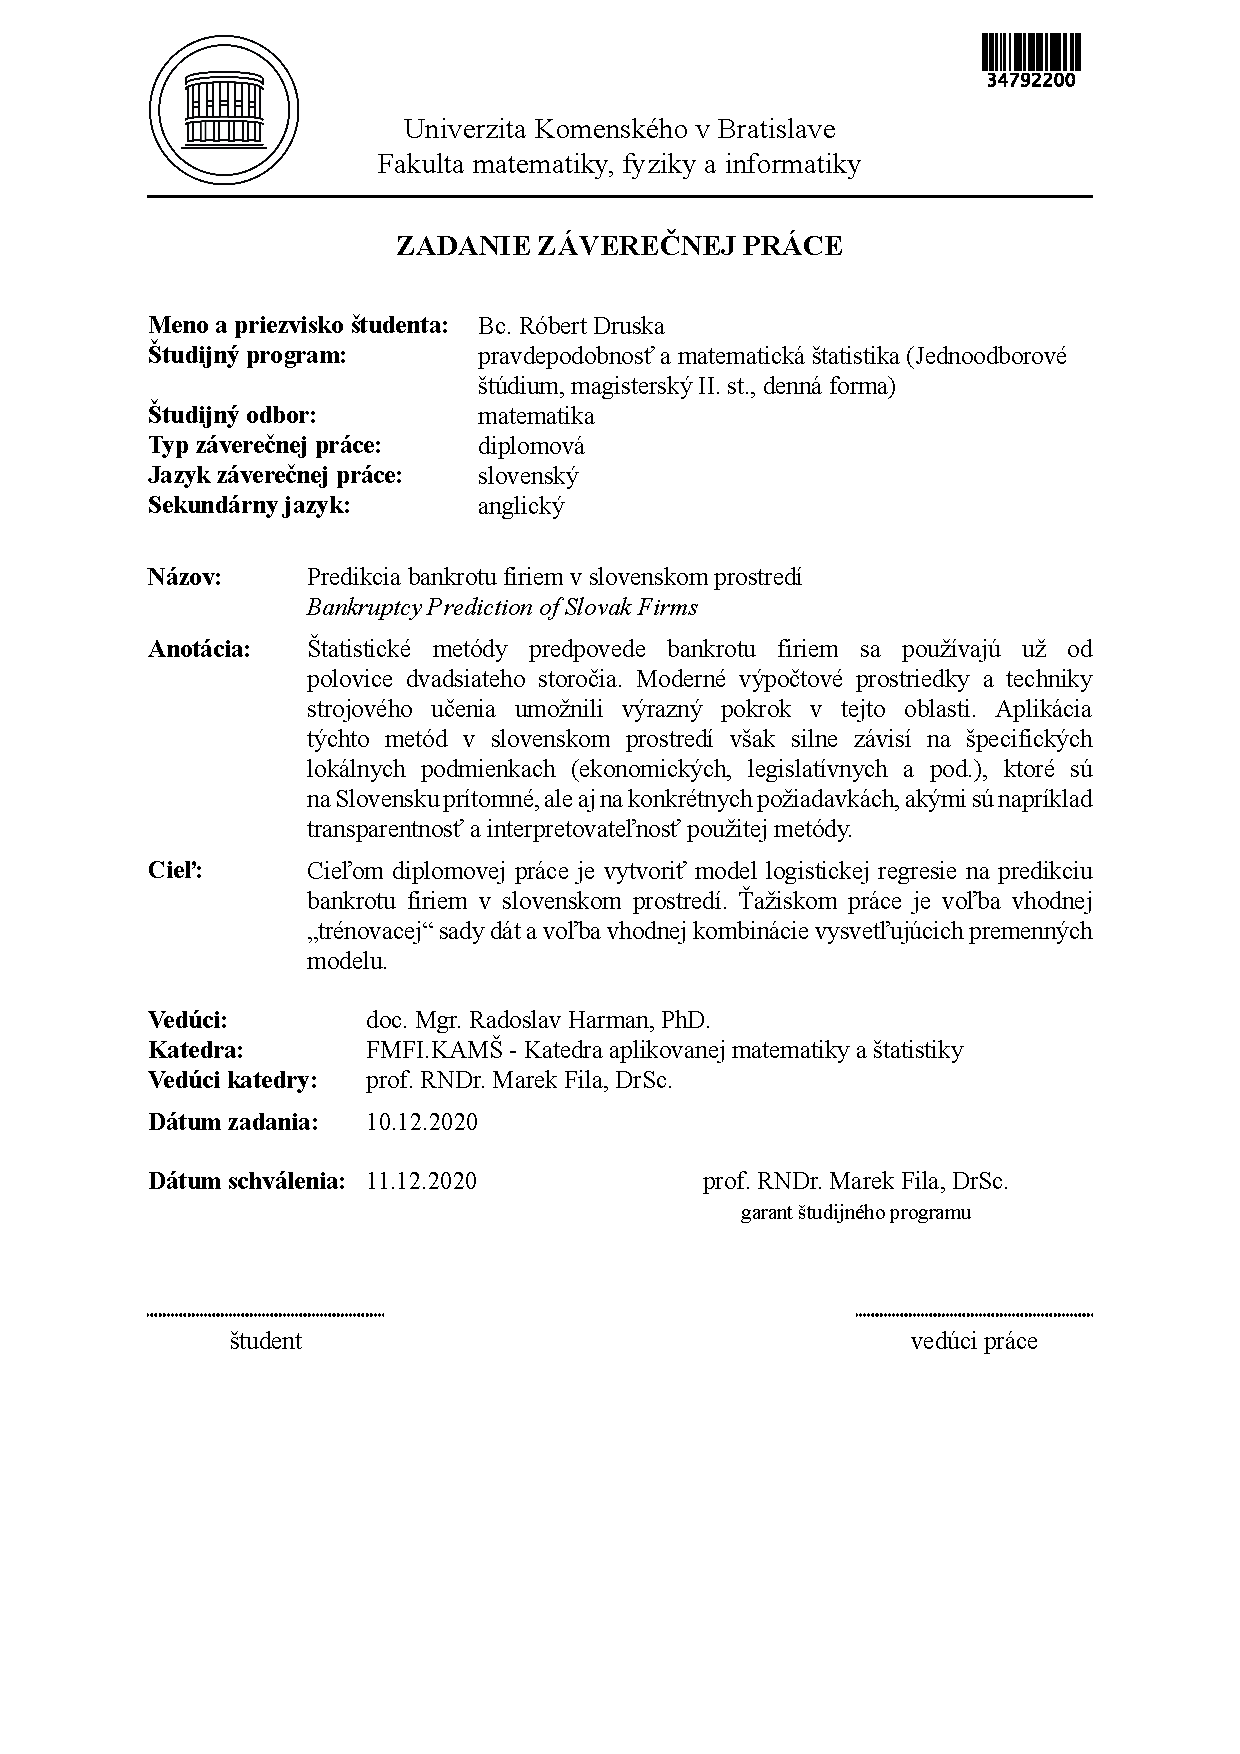
\includepdf[pages={1}, offset=25 -75]{zadanieRD.pdf}

  

\vglue0pt
\vfill
\thispagestyle{empty}
\paragraph{Poďakovanie}

Touto cestou by som sa chcel poďakovať svojmu školiteľovi, Radoslavovi Harmanovi, za jeho ochotu a množstvo dobrých a pravidelných rád pri písaní tejto práce.
Ďakujem tiež svojej kolegyni Monike Hrnčárovej za cenné analýzy predchádzajúce praktickým častiam práce, a svojej mame za gramatickú a štylistickú korektúru.
V neposlednom rade ďakujem svojim priateľom za oporu v posledných mesiacoch písania.


  \newpage
  \thispagestyle{empty}
\section*{Abstrakt}
DRUSKA, Róbert: Predikcia úpadku slovenských firiem [Diplomová práca],
Univerzita Komenského v Bratislave,
Fakulta matematiky, fyziky a informatiky,
Katedra aplikovanej matematiky a štatistiky,
školiteľ: doc. Mgr. Radoslav Harman, PhD.,
Bratislava, 2020, TODO s.

TODO Lorem ipsum dolor sit amet, consectetur adipiscing elit, sed do eiusmod tempor incididunt ut labore et dolore magna aliqua. Ut enim ad minim veniam, quis nostrud exercitation ullamco laboris nisi ut aliquip ex ea commodo consequat. Duis aute irure dolor in reprehenderit in voluptate velit esse cillum dolore eu fugiat nulla pariatur. Excepteur sint occaecat cupidatat non proident, sunt in culpa qui officia deserunt mollit anim id est laborum.

\begin{flushleft}
  \textbf{Kľúčové slová:} logistická regresia, TODO
\end{flushleft}

  \newpage
  \thispagestyle{empty}
\section*{Abstract}
DRUSKA, Róbert: Bankruptcy prediction [Master thesis],
Comenius University in Bratislava,
Faculty of Mathematics, Physics and Informatics,
Department of Applied Mathematics and Statistics,
supervisor: doc. Mgr. Radoslav Harman, PhD.,
Bratislava, 2020, TODO p.

TODO Lorem ipsum dolor sit amet, consectetur adipiscing elit, sed do eiusmod tempor incididunt ut labore et dolore magna aliqua. Ut enim ad minim veniam, quis nostrud exercitation ullamco laboris nisi ut aliquip ex ea commodo consequat. Duis aute irure dolor in reprehenderit in voluptate velit esse cillum dolore eu fugiat nulla pariatur. Excepteur sint occaecat cupidatat non proident, sunt in culpa qui officia deserunt mollit anim id est laborum.

\begin{flushleft}
  \textbf{Keywords:} logistic regression, TODO
\end{flushleft}
  \newpage \tableofcontents
  \setcounter{page}{7}
 % \newpage
 % \listoffigures
 % \newpage
 % \listoftables  
  \newpage

    \section*{Úvod}	          
    \markboth{ÚVOD}{ÚVOD}  
    \addcontentsline{toc}{section}{Úvod}
    
    Predikcia bankrotu firiem je predmetom akademického aj profesionálneho výskumu už po dlhé desaťročia.
Motivácia stojaca za hľadaním modelov na predikciu úpadku firiem je rôzna.
Prvé modely vytvorené na základe dát o verejne obchodovateľných spoločnostiach v USA
boli využívané pri analýzach predchádzajúcich nákupom akcií \cite{altman1968}.
Modely kreditného rizika našli veľké využitie v bankovníctve – banky a iné finančné inštitúcie disponujú internými modelmi,
ktorými vyhodnocujú finančnú kondíciu svojich klientov a ich hodnotenia využívajú napr. pri stanovovaní úrokových sadzieb.
Takisto aj súkromné spoločnosti a živnostníci môžu využiť modely kreditného rizika pri bežnom vykonávaní svojej podnikateľskej praxe.

V prvých dvoch kapitolách sa oboznamujeme s problematikou bankrotu na Slovenku a predstavíme si dva známe modely kreditného rizika – Altmanovo Z-skóre a český index IN05.
Tretia kapitola je teoretickou predprípravou k metodike,
ktorú sme v práci použili na modelovanie predikcie bankrotu v slovenskom prostredí.
Oboznámime sa v nej s logistickou regresiou a tiež s metódou \emph{BACE}, ktorá slúži na výber vhodnej kombinácie parametrov do modelu.
V štvrtej kapitole sa bližšie venujeme metodike praktickej časti práce.

V piatej kapitole dôkladne opíšeme proces vytvorenia modelov predikcie bankrotu
od popisu dát cez technické detaily modelovania až po porovnanie nami vytvorených modelov s Altmanovým Z-skóre a indexom IN05
aj medzi sebou navzájom. Posledná, šiesta kapitola obsahuje diskusiu o interpretácii výstupov bankrotových modelov. 

    \newpage
    \section{Bankrot na Slovensku}
\label{bankruptcy}

Cieľom tejto práce je vytvoriť model na predikciu úpadku firiem na základe jej finančných údajov.
Pre účely modelovania si na začiatok zadefinujme, čo budeme rozumieť pod pojmom úpadok.
Problematikou bankrotu právnických a fyzických osôb na Slovensku sa venuje najmä zákon 7/2005 Z. z. o konkurze a reštrukuturalizácii \cite{zbierkazakonov},
ktorý definuje úpadok nasledovne.

\bigskip
\textit{(1)
Dlžník je v úpadku, ak je platobne neschopný alebo predlžený. Ak dlžník podá návrh na vyhlásenie konkurzu, predpokladá sa, že je v úpadku.}

\textit{(2)
Právnická osoba je platobne neschopná, ak nie je schopná plniť 30 dní po lehote splatnosti aspoň dva peňažné záväzky viac ako jednému veriteľovi. […]}

\textit{(3)
Predlžený je ten, kto je povinný viesť účtovníctvo podľa osobitného predpisu, má viac ako jedného veriteľa a hodnota jeho záväzkov presahuje hodnotu jeho majetku. […]}
\bigskip

Keď je právnická osoba v úpadku, je potrebné vyhlásiť konkurz alebo reštrukturalizáciu.
Konkurzné a reštrukturalizačné konania schvaľuje súd, vďaka čomu poznáme presný dátum ich začiatku, čo sa nám zíde pri modelovaní.

Konkurz znamená speňaženie majetkovej podstaty dlžníka a pomerné uspokojenie jeho veriteľov z tohto majetku.
Konkurz má charakter likvidačného konania a jeho výsledkom je zrušenie a zánik podniku.
V bežnej praxi ide o zdĺhavý proces, ktorý môže trvať aj niekoľko rokov.

Na rozdiel od konkurzu reštrukturalizácia nemá likvidačný charakter a je možné vyhlásiť ju už v čase hroziaceho úpadku.
Cieľom reštrukturalizácie je zachovanie podniku alebo jeho časti a postupné uspokojenie veriteľov spôsobom dohodnutým v reštrukturalizačnom pláne.
Uspokojenie pohľadávok býva v praxi rýchlejšie ako pri konkurze.
V prípade, že reštrukturalizácia bude úspešná, právnická osoba može naďalej pokračovať v podnikateľskej činnosti,
avšak predpokladom jej úspechu je to, že pohľadávky veriteľov sa budú počas ďalšieho fungovania podniku uspokojovať vo vyššej miere ako v prípade konkurzu.

Spoločným znakom konkurzu a reštrukturalizácie je skutočnosť, že dlžník sa nachádza v krízovej ekonomickej situácii.
Pre účely tejto práce budeme \emph{bankrotom} rozumieť začiatok konkurzného alebo reštrukturalizačného konania.

\subsection{Bankrot - vzácna udalosť}

Úpadok alebo bankrot možno považovať v rámci populácie aktívnych firiem za vzácnu udalosť.
Databáza \emph{FinStat}, ktorej dáta budeme využívať v tejto práci, eviduje celkovo 6946 prípadov konkurzného alebo reštrukturalizačného konania za obdobie existencie samostatnej Slovenskej republiky.
Ako uvidíme, nie každé z týchto konaní sa hodí na modelovanie, či už kvôli nedostatku dostupných dát alebo inej príčiny.

Napríklad, z počtu 6946 firiem v úpadku len pre 3730 firiem poznáme presný dátum začiatku konkurzného alebo reštrukturalizačného konania.
Dátum začiatku konania nepoznáme zväčša pre staršie firmy, ktoré zanikli pred rokom 2010, a pre ktoré by sme v mnohých prípadoch aj tak nemali dostatok dát pre úspešné zahrnutie do modelu.

V tabuľke uvádzame počet konkurzov a reštrukturalizácií a počet aktívnych firiem od roku 2011 po rok 2020.

\begin{center}
    \begin{tabular}{ |c|c|c|c|p{3cm}|p{3cm}| }
        \hline
        Rok & Konkurzy & Reštrukturalizácie & Spolu & Celkový počet aktívnych firiem & Proporcia firiem v úpadku \\
        \hline
        2011 & 282 & 21 & 303 & TODO & TODO \\
        \hline
        2012 & 296 & 36 & 332 & & \\
        \hline
        2013 & 318 & 49 & 367 & & \\
        \hline
        2014 & 329 & 56 & 385 & & \\
        \hline
        2015 & 325 & 49 & 374 & & \\
        \hline
        2016 & 222 & 35 & 257 & & \\
        \hline
        2017 & 215 & 22 & 237 & & \\
        \hline
        2018 & 256 & 6 & 262 & & \\
        \hline
        2019 & 254 & 8 & 262 & & \\
        % pozn: v roku 2019 mala jedna firma konanie s kategoriou "ine", ide o firmu s ico 36595098 ... po rucnej kontrole som ju zaradil medzi restrukturalizacie
        \hline
        2020 & 185 & 19 & 204 & & \\
        \hline
    \end{tabular}
\end{center}
\bigskip

Ako vidíme, počet firiem v úpadku sa každoročne nachádza pod hranicou 0,5 \% z aktívnych firiem.
Z uvedeného vyplýva, že pri modelovaní úpadku firiem budeme pracovať so silno nevyváženými dátami (angl. \emph{angl. unbalanced classes}).
Napriek tomu, že bankrot je v populácii firiem vzácny, ide o udalosť, ktorej predpovedanie je zaujímavé pre množstvo strán -
napr. pre manažment firiem, majiteľov firemného kapitálu, poskytovateľov pôžičiek, investorov či poisťovateľov.

TODO: bližší opis bankrotov podľa odvetví, veľkosti firiem, potenciálne niečo o vplyve covid pandémie atď. a pod.,
dá sa tu spraviť veľa deskriptívnej štatistiky

    \newpage
    \section{Známe bankrotové modely}

Riziko úpadku podnikov sa modeluje už desiatky rokov.
Za jeden z prvých formálnych pokusov o štatistickú analýzu úpadku podnikov je považovaná štúdia FitzPatricka z roku 1932 \cite{fitzpatrick},
v ktorej autor pracoval s dátami o 40 firmách (20 v úpadku, 20 zdravých).
Výsledkom FitzPatrickovej štúdie nebol model rizika úpadku, ale analýza jednotlivých finančných ukazovateľov a ich trendov pri prosperujúcich a neprosperujúcich firmách.

Formálnejšie pokusy o modelovanie rizika úpadku firiem začali v 60. rokoch, keď vznikli napr. modely Beavera \cite{beaver}, Tamariho \cite{tamari} alebo Altmana \cite{altman1968},
ktorého Z-skóre vytvorené metódou diskriminačnej analýzy patrí dodnes medzi najpoužívanejšie modely kreditného rizika.
Diskriminačná analýza prevažovala v rámci metód používaných na modelovanie úpadku podnikov až do 80. rokov, keď ju nahradili metódy,
ktoré majú menej matematických požiadaviek na dáta, ako napr. logistická regresia alebo \emph{probit model} \cite{gruszczynski}.

Rozmach moderných technológií, výpočtovej techniky a ľahší prístup k dátam v 21. storočí umožnili použitie mnohých ďalších metód na modelovanie kreditného rizika.
V literatúre vieme nájsť modely neurónovej siete \cite{tsai}, hazardné modely \cite{shumway}, metódu oporných bodov (SVM) \cite{min} atď.

Známe sú aj modely vytvorené pomocou dát o slovenských a českých firmách, napr. bonitné indexy IN vytvorené manželmi Neumaierovými na dátach o českých firmách
či Binkertov model \cite{zalai} slovenského prostredia.
Na tému analýzy kreditného rizika firiem tiež vzniklo niekoľko záverečných prác na FMFI UK \cite{ondrusekova, bohdal}.

\subsection{Altmanovo Z-skóre}

Altmanovo \(Z\)-skóre patrí historicky k najznámejším a najpoužívanejším modelom predikcie bankrotu.
Prvá verzia \(Z\)-skóre bola vytvorená na vzorke \(66\) verejne obchodovateľných firiem, \(33\) prosperujúcich a \(33\) v úpadku \cite{altman1968}.
Išlo o model viacrozmernej diskriminačnej analýzy
\footnote{V anglickej literatúre sa o metóde využitej pri Altmanovom modeli hovorí ako o \emph{multivariate discriminant analysis} (MDA).}
s \(5\) premennými predstavujúcimi finančné údaje o firme.
Vzorku 33 prosperujúcich firiem zvolil Altman tak, že ku každej z \(33\) firiem v úpadku zvolil firmu podobnej veľkosti pôsobiacu v rovnakom odvetví ako daná firma v úpadku.
Pri vzorke firiem v úpadku používal údaje jeden rok pred vyhlásením bankrotu, pri dopárovaných prosperujúcich firmách používal údaje z toho istého roku.

Pôvodná verzia \(Z\)-skóre pracovala s trhovou hodnotou firmy, ktorá je dostupná len pre verejne obchodovateľné spoločnosti. Jej tvar je nasledovný:

\[
    Z = 0.012X_1 + 0.014X_2 + 0.033X_3 + 0.006X_4 + 0.999X_5,
\]

kde

\(X_1 = \) pracovný kapitál / aktíva,

\(X_2 = \) výsledok hospodárenia minulých rokov\footnote{angl. \emph{retained earnings}} / aktíva,
% nerozdelený zisk

\(X_3 = \) EBIT\footnote{zisk pred zdanením a úrokmi (angl. \emph{earnings before interest and taxes})} / aktíva,

\(X_4 = \) trhová hodnota / celkové záväzky,

\(X_5 = \) tržby / aktíva.
\bigskip

Podľa modelu je spoločnosť v prosperujúcej zóne, ak \(Z > 2.99\), a v úpadku, ak \(Z < 1.81\).
Interval \([1.81, 2.99]\) nazývame „šedou“ zónou – ak má firma hodnotu \(Z\) v danom intervale, model firmu jednoznačne nezaraďuje do žiadnej z dvoch skupín
(prosperujúca firma alebo firma v úpadku).

Ako bolo zdôraznené v \cite{altman1983}, pôvodné \(Z\)-skóre bolo vytvorené na vzorke verejne obchodovateľných spoločností a je aplikovateľné len na tento typ firiem.
Pokusom o \emph{ad hoc} modifikáciu modelu (napr. nahradením trhovej hodnoty vlastným imaním) chýbala vedecká exaktnosť.
V roku 1983 vytvoril Altman novú verziu \(Z\)-skóre, aplikovateľnú aj na súkromné spoločnosti, v tvare:

\[
    Z = 0.717X_1 + 0.847X_2 + 3.107X_3 + 0.420X_4 + 0.998X_5,
\]

kde \(X_4 = \) trhová hodnota / celkové záväzky, a ostatné premenné majú rovnaký význam ako v pôvodnom \(Z\)-skóre z roku 1968.

Hranice intervalov pre modifikované \(Z\)-skóre sú:

\( Z > 2.9\) – prosperujúca zóna,

\( Z \in [1.2, 2.9]\) – šedá zóna,

\( Z < 1.2 \) – zóna úpadku.
\bigskip

Keďže väčšina firiem na Slovensku je v súkromnom vlastníctve, v slovenskom prostredí sa využíva hlavne verzia Altmanovho skóre z roku 1983.
Presnosť modelov vytvorených v tejto práci budeme porovnávať práve s touto verziou \(Z\)-skóre.

Aj autor \(Z\)-skóre Edward Altman uznal, že presnosť jeho modelu bola prekonaná inými, konkurenčnými modelmi \cite{altman2017}, napriek tomu však \(Z\)-skóre patrí medzi najpoužívanejšie modely predikcie bankrotu.
Dôvodmi pre túto skutočnosť sú zrejme jednoduchosť a ľahká interpretovateľnosť jeho vzorca a dostatočne vysoká presnosť modelu v globálnom prostredí
(v \cite{altman2017} Altman ukazuje, že presnosť klasifikácie pre väčšinu krajín je vyššia než približne \(0.75\)).


\subsection{Index IN05}

Index IN05 (viď \cite{neumaier1}) je český model slúžiaci na ohodnotenie finančného zdravia spoločnosti.
Model patrí do skupiny bonitných indexov IN vytvorených manželmi Neumaierovými, pričom index IN05 je najnovší z nich a pochádza z roku 2005.
Podobne ako Altmanovo Z-skóre, tento model vznikol na základe diskriminačnej analýzy. Diskriminačná funkcia indexu IN05 má tvar:

\[
    \text{IN05} = 0.13X_1 + 0.04X_2 + 3.97X_3 + 0.21X_4 + 0.09X_5,
\]

kde

\(X_1 = \) aktíva / cudzie zdroje,

\(X_2 = \) EBIT / nákladové úroky,

\(X_3 = \) EBIT / aktíva,

\(X_4 = \) výnosy / aktíva,

\(X_5 = \) obežné aktíva / (krátkodobé závazky + bežné bankové úvery).
\bigskip

Hranice intervalov pre hodnoty indexu IN05 sú:

\( \text{IN05} > 1.6\) – prosperujúca zóna,

\( \text{IN05} \in [0.9, 1.6]\) – šedá zóna,

\( \text{IN05} < 0.9 \) – zóna úpadku.
\bigskip

Podľa publikácie \cite{sav} má pri identifikácii bankrotu index IN05 úspešnosť \(77 \%\), ktorá bola nameraná na vzorke \( 1526 \) českých podnikov.



    \newpage  
    \section{Teoretická predpríprava}
\label{teoreticka predpriprava}

\subsection{Logistická regresia}
 
Logistická regresia je štatistická metóda využívaná pri binárnej klasifikácii, resp. pri predikcii náhodného binárneho výsledku.
Cieľom logistickej regresie je modelovať pravdepodobnosť nejakej triedy alebo udalosti (vysvetľovanej premennej)
na základe jednej alebo viacerých vysvetľujúcich premenných. TODO

Pred tým, než opíšeme, ako presne logistická regresia funguje, si zadefinujme niekoľko dôležitých pojmov, s ktorými logistická regresia narába.

\begin{defin}
    Logistická funkcia \( \sigma : \mathbb{R} \rightarrow (0, 1) \) je definovaná ako:
    \[
        \sigma(t) = \frac{e^t}{e^t + 1} = \frac{1}{1 + e^{-t}}.
    \]
    Inverzná funkcia k logistickej sa nazýva logit funkcia a spĺňa:
    \[
        logit(t) = \sigma^{-1}(t) = \ln\left(\frac{p}{1 - p}\right),
    \]
    pre \( p \in (0, 1) \).
\end{defin}

Na obrázku je zobrazený graf logistickej funkcie na intervale \( (-6, 6) \):

% \begin{center}
%     \begin{tikzpicture}
%     \begin{axis}[
%         xlabel={x},
%         ylabel={y},
%         xmin=-6, xmax=6,
%         ymin=0, ymax=1,
%         xtick={-4,-2,0,2,4},
%         ytick={0,0.2,0.4,0.6,0.8,1},
%         legend pos=north west,
%         ymajorgrids=true,
%         grid style=dashed,
%         height=8cm,
%         width=15cm,
%     ]
    
%     \addplot[
%         color=blue,
%         mark=square,
%         ]
%         coordinates {
%         (2, 1.0)(3, 0.5)(4, 0.25)(5, 0.16667)(6, 0.11111)(7, 0.08333)(8, 0.0625)(9, 0.05)(10, 0.04)(11, 0.03333)(12, 0.02778)(13, 0.02381)(14, 0.02041)(15, 0.01786)(16, 0.015625)
%         };
%         % \legend{Rozptyl}
        
%     \end{axis}
%     \end{tikzpicture}
% \end{center}


\begin{center}
\begin{tikzpicture}[>=stealth]
    \begin{axis}[
        xmin=-6,xmax=6,
        ymin=0,ymax=1,
        axis x line=middle,
        axis y line=middle,
        axis line style=<->,
        xlabel={$x$},
        ylabel={$y$},
        ]
        \addplot[no marks,blue,solid] expression[domain=-6:6,samples=100]{1/(1 + exp(-x))};
    \end{axis}
\end{tikzpicture}
\end{center}

Argumentom prirodzeného logaritmu v logit funkcii je výraz \( \frac{p}{1 - p} \) pre \( p \in (0, 1) \).
Ak takéto \(p\) budeme chápať ako pravdepodobnosť, výraz \( \frac{p}{1 - p} \) predstavuje takzvaný pomer šancí (\emph{angl. odds-ratio}).
Napríklad pri hode kockou je pravdepodobnosť padnutia šestky rovná \( 1/6 \) a pomer šancí je \( \frac{\frac{1}{6}}{1 - \frac{1}{6}} = \frac{\frac{1}{6}}{\frac{5}{6}} = \frac{1}{5} = 1 : 5\),
čo znamená, že 1 možný výsledok hodu kockou zodpovedá šestke a 5 možných výsledkov šestke nezodpovedá.

Nech \( Y \) je binárna vysvetľovaná premenná, ktorej zodpovedá vektor vysvetľujúcich premenných \( x = (1, x_1, x_2, \ldots, x_k) \)
(jednotka na začiatku bude v modeli logistickej regresie zodpovedať hodnote \emph{interceptu}).
Pre \( Y \) zjavne platí \( P(Y = 1|x) = 1 - P(Y = 0|x) \).
Logistická regresia predpokladá, že logaritmus pomeru šancí (angl. \emph{log-likelihood ratio}) možno modelovať ako lineárnu funkciu zložiek vektora \( x \).

\[
\ln \left( \frac{P(Y = 1|x)}{P(Y = 0|x)} \right) = \ln \left( \frac{P(Y = 1|x)}{1 - P(Y = 1|x)} \right) = \beta_0 + \beta_1 x_1 + \beta_2 x_2 + \ldots + \beta_k x_k = \beta^T x.
\]

Po úpravách sa ľahko dopracujeme k záveru, že pravdepodobnosť \( P(Y = 1|x) \) je rovná výstupu logistickej funkcie, ktorej argument bude hľadaná lineárna kombinácia zložiek vektora \( x \).

\begin{equation} \label{logistic_regression}
P(Y = 1|x) = \frac{1}{1 + e^{-\beta^T x}} := h_\beta(x).
\end{equation}

Inými slovami, logistická regresia predpokladá, že pre vektor vysvetľujúcich premenných \(x\) má pozorovanie \(Y\)
alternatívne (Bernoulliho) rozdelenie s parametrom \(h_\beta(x)\).
Ak logistickú regresiu používame na predikciu (čo budeme robiť neskôr v tejto práci),
vzorec (\ref{logistic_regression}) nám poslúži na výpočet pravdepodobnosti \( P(Y = 1|x) \) pri danom novom \( x \).

\subsubsection{Odhad parametrov v logistickej regresii}

Majme teda zovšebecnený regresný model tvaru

\[
h_\beta(x) = P(Y = 1|x) = \frac{1}{1 + e^{-\beta^T x}}
\]

Neznámym parametrom v tomto modeli je koeficient \( \beta = (\beta_0, \beta_1, \ldots, \beta_k) \).
Na odhad parametra \( \beta \) sa vo väčšine prípadov používa metóda maximálnej vierohodnosti.
Na rozdiel od obyčajnej lineárnej regresie s normálne rozdelenými chybami,
v logistickej regresii nie je možné nájsť exaktné analytické vyjadrenie odhadu parametra \( \beta \) metódou maximálnej vierohodnosti
a pre konkrétne dáta sa na výpočet tohto odhadu používa nejaká iteračná metóda.

Keďže \(Y\) nadobúda len hodnoty z \( \{0, 1\} \), pre vierohodnostnú funkciu \(Y\) platí:

\[
P(y | x; \beta ) = h_\beta(x)^y (1 - h_\beta(x))^{1 - y}
\]

Majme namerané vektory dát \( x_1, \ldots, x_n \), kde \( x_i = (1, x_{i1}, \ldots, x_{ik}) \),
a k nim prislúchajúci vektor nameranej vysvetľovanej premennej \(y = (y_1, \ldots, y_n )\). Označme

\[
    X =
    \left[
        \begin{array}{ccc}
            \horzbar & x_{1} & \horzbar \\
            \horzbar & x_{2} & \horzbar \\
                    & \vdots    &          \\
            \horzbar & x_{n} & \horzbar
        \end{array}
    \right].
\]


Potom pre funkciu vierohodnosti parametra \( \beta \) platí

\[
L(\beta | X, y) = \prod_{i = 1}^n h_\beta(x_i)^{y_i} (1 - h_\beta(x_i))^{1 - y_i}
\]

Trénovanie logistickej regresie spočíva v maximalizovaní funkcie vierohodnosti,
čo je ekvivalentné maximalizácii jej logaritmu (angl. \emph{log-likelihood function}), a teda hľadáme

\[
\hat{\beta} := \max_{\beta} \ln L(\beta | y) = \max_{\beta} \sum_{i = 1}^n y_i \ln{h_{\beta}(x_i)} + (1 - y_i) \ln{(1 - h_{\beta}(x_i))}
\]

Na nájdenie maxima log-likelihood funkcie v prípade logistickej regresie sa používajú iteračné metódy,
napr. funkcia \emph{glm} v základnej verzii jazyka \emph{R} využíva metódu \emph{IRLS} (\emph{iteratively reweighted least squares}).

\subsubsection{Sumárne štatistiky v logistickej regresii}

TODO: Tu napíšem niečo o hodnotách ako \(R^2\) atď., ešte to nemám celkom premyslené.

\subsubsection{Interpretácia parametrov v logistickej regresii}

TODO

\subsection{Bayesian averaging of classical estimates (BACE)}

Dáta, ktoré budeme spracúvať v našej práci, obsahujú 70 vysvetľujúcich premenných pre každý rok pôsobenia firmy.
Prirodzene, nie všetky z nich sa hodia na modelovanie bankrotu.
Naším cieľom bude vytvoriť model, ktorý bude relatívne jednoduchý, a v ktorom budú vystupovať len tie najsignifikantnejšie vysvetľujúce premenné z hľadiska predikcie bankrotu.
V tejto časti si opíšeme jednu z metód, ktorú použijeme, a to \emph{Bayesian averaging of classical estimates} (\emph{BACE}).

Základná metóda \emph{BACE} bola vybudovaná za účelom vytvorenia lineárnej regresie, ale jej hlavnú ideu možno ľahko využiť aj pri logistickej regresii.
Názov \emph{Bayesian averaging of classical estimates} vznikol na základe toho, že metóda BACE využíva bayesovské priemerovanie modelov (angl. \emph{Bayesian averaging}) a klasické odhady parametrov lineárnej regresie metódou najmenších štvorcov.

\subsubsection{Bayesovská štatistika}

Metóda \emph{BACE} narába s teóriou bayesovskej štatistiky.
V klasickej štatistike predpokladáme, že parametre majú pevnú, ale neznámu hodnotu.
Neznáme parametre v klasickej štatistike nie sú náhodnými premennými a nemajú pravdepodobnostnú hustotu.
Narozdiel od toho v bayesovskej štatistike považujeme parametre za náhodné premenné, pričom ich náhodnosť zodpovedá miere neistoty, ktorú o danom parametri máme.

\subsubsection{Bayesovské priemerovanie modelov (\emph{Bayesian model averaging})}

Jedným zo základných tvrdení bayesovskej štatistiky je tzv. Bayesovo pravidlo, ktoré hovorí nasledovne:

\[
P(A|B) = \frac{P(B|A) P(A)}{P(B)}.
\]

Bayesovo pravidlo možno zovšeobecniť pre spojité náhodné premenné a ich hustoty. Pre náhodné premenné \(y\) a \( \beta \) platí:

\begin{equation} \label{bayes_rule}
    g(\beta | y) = \frac{f(y | \beta) g(\beta)}{f(y)}.
\end{equation}

Aplikujme vzorec (\ref{bayes_rule}) na premenné, ktoré vystupujú v logistickej regresii.
Nech \( \beta \) je vektor parametrov (intercept a koeficienty jednotlivých vysvetľujúcich premenných),
\( g(\beta) \) je jeho apriórna hustota, ktorú interpretujeme ako presvedčenie výskumníka o parametri \( \beta \) predtým, než spoznáme dáta,
\( y \) nech je vektor nameraných dát a \( f(y) \) jeho hustota.
\( g(\beta | y) \) je aposteriórna hustota parametra \( \beta \) (hustota podmienená nameranými dátami \( y \)) a predstavuje presvedčenie výskumníka o parametri \( \beta \) po tom, ako spoznáme dáta \( y \).
Bayesovo pravidlo hovorí o tom, ako skombinovať apriórnu informáciu \( g \) s nameranými dátami \( y \) a spočítať naše konečné presvedčenie o parametri \( \beta \) – jeho aposteriórnu hustotu \( g(\beta|y) \).

Majme množinu \( X = \{X_1, \ldots,  X_k\} \) potenciálnych vysvetľujúcich premenných pre model logistickej regresie.
Pri skúmaní signifikantnosti jednotlivých premenných \( X_1, \ldots, X_k \) máme možnosť danú premennú do modelu zaradiť alebo nezaradiť,
existuje teda celkovo \( 2^k \) modelov so všetkými možnými kombináciami vysvetľujúcich premenných \( X_1, \ldots, X_k \).
(\( M_i \) môže byť reprezentované napr. binárnym vektorom dĺžky \(k\), pričom hodnota na mieste \( j = 1, \ldots, k \) hovorí o zaradení, resp. nezaradení \(j\)-tej vysvetľujúcej premennej do modelu.)

Výskumník zvolí apriórne pravdepodobnosti \( p(M_i) \), pričom \( \sum p(M_i) = 1 \) (problematikou voľby apriórnych pravdepodobností sa budeme zaoberať neskôr).
Z bayesovho pravidla vyplýva, že:

\[
    g(\beta | y) = \sum_{i = 1}^{2^k} p(M_i) \frac{f(y | \beta) g(\beta | M_i)}{f(y)}.
\]

Pre aposteriórne pravdepodobnosti vyzerá vzorec nasledovne:

\begin{equation} \label{posterior_probabilities}
    g(\beta | y) = \sum_{i = 1}^{2^k} p(M_i | y) \frac{f(y | \beta) g(\beta | M_i)}{f(y | M_i)},
\end{equation}

kde \(p(M_i|y)\) je aposteriórna pravdepodobnosť modelu \(M_i\) po tom, čo spoznáme dáta \(y\).
Vzorec (\ref{posterior_probabilities}) hovorí, že aposteriórne rozdelenie parametra \(\beta\) je váženým priemerom aposteriórnych hustôt parametra beta podmienených modelom \(M_i\),
s váhami rovnými aposteriórnym pravdepodobnostiam modelov \(M_i\).
Takýto prístup zakomponovania neistôt modelov do výpočtu hľadanej veličiny sa nazýva \emph{Bayesian model averaging} (\emph{BMA}).

Keď poznáme aposteriórne pravdepodobnosti (resp. váhy) modelov \( M_i \), umožní nám to výpočet strednej hodnoty parametra \( \beta \):

\begin{equation} \label{posterior_expected_value}
    E(\beta | y) = \sum_{i = 1}^{2^k} p(M_i | y) \hat{\beta}^{(i)},
\end{equation}

kde \( \hat{\beta}^{(i)} = E(\beta |y, M_i) \) je odhad parametra \( \beta \) pri použití modelu \( M_i \) metódou maximálnej vierohodnosti
(pozn.: pôvodná metóda BACE pracovala s lineárnou regresiou, kde odhad metódou maximálnej vierohodnosti je vlastne jednoznačný \emph{klasický} odhad metódou najmenších štvorcov;
v prípade logistickej regresie parameter odhadujeme iteračnou metódou).

Aposteriórna disperzia parametra beta je daná vzorcom:

\[
    D(\beta | y) = \sum_{i = 1}^{2^k} p(M_i | y) D(\beta | y, M_i) + \sum_{i = 1}^{2^k} p(M_i | y) \left( \hat{\beta}^{(i)} - \sum_{i = 1}^{2^k} p(M_i | y) \hat{\beta}^{(i)} \right)^2.
\]

Poznanie aposteriórnych hustôt modelov navyše umožňuje výpočet aposteriórnej pravdepodobnosti zahrnutia premennej do modelu (\emph{angl. posterior inclusion probability}),
čo bude jednoducho súčet aposteriórných pravdepodobností modelov obsahujúcich danú vysvetľujúcu premennú:

\begin{equation} \label{posterior_inclusion_probability}
    p(\beta_j \neq 0 | y) = \sum_{i = 1}^{2^k} p(M_i | y) I_{\beta_{j, i} \neq 0},
\end{equation}

kde \( I_{\beta_{j, i} \neq 0} \) je indikátor prítomnosti vysvetľujúcej premennej \( X_j \) v modeli \( M_i \).

Výpočet aposteriórnej pravdepodobnosti zahrnutia bude hlavný výstup metódy BACE, ktorý využijeme.
Za signifikantné premenné označíme tie, ktorých aposteriórna pravdepodobnosť zahrnutia bude vyššia ako apriórna pravdepodobnosť zahrnutia, čo predstavuje štandardný postup pri využívaní tejto metódy pri regresiách.

Teória za bayesovským priemerovaním modelov je priamočiara,
ale jeho praktická implementácia prináša dve hlavné výzvy – voľbu apriórnych pravdepodobnosti modelov a dopočitanie ich aposteriórnych pravdepodobností.

\subsubsection{Voľba apriórnych pravdepodobností}

Sila bayesovskej štatistiky spočíva v tom, že nám pri odhadoch hľadanej veličiny dáva možnosť využiť naše apriórne presvedčenie o nej – jej apriórne rozdelenie.
Ukazuje sa, že táto „prednosť“ bayesovskej štatistiky je zároveň problémom, pretože voľba apriórnych pravdepodobností býva často náročná úloha.
Apriórne rozdelenia sa zvyčajne volia na základe informácií z predošlých štúdií zaoberajúcich sa danou problematikou alebo názorov expertov z danej oblasti \cite{carlin}.
Pri výbere apriórneho rozdelenia sa často volí rozdelenie z nejakej známej triedy, napr. normálne, binomické, poissonovo atď.

Pri veľkom množstve parametrov je väčšinou nepraktické voliť apriórne rozdelenie pre každý jeden z nich.
V podobných prípadoch sa zvykne voliť apriórne rozdelenie, ktoré má neinformatívny charakter, napr. rôzne varianty rovnomerného rozdelenia.
V takom prípade sú primárnym zdrojom informácie dáta, podobne ako pri bežnej frekventistickej (angl. \emph{frequentist}) štatistike \cite{tiao}.

V situácii, keď princípy bayesovskej štatistiky využívame na výber vhodnej kombinácie premenných pre regresný model,
nebudeme voliť apriórne rozdelenia pre samotné koeficienty regresného modelu, ale pre pravdepodobnosť ich zahrnutia do modelu.
Podobne ako autori metódy BACE rovnomerne zvolíme apriórnu pravdepodobnosť zahrnutia (angl. \emph{prior inclusion probability}) pre všetky premenné,
s ktorými pracujeme. Všetky premenné dostanú rovnakú apriórnu pravdepodobnosť zahrnutia.

Jediná apriórna informácia, ktorú ako výskumníci vložíme do nášho skúmania,
je samotná hodnota apriórnej pravdepodobnosti zahrnutia premenných.
Pri jej voľbe využijeme očakávaný počet premenných vo výslednom modeli.
Ak pri celkovom počte premenných \(K\) označíme priemerný očakávaný počet premenných vo výslednom modeli \(\bar{k}\) a zahrnutie každej dvojice premenných budeme považovať za nezávislé,
apriórna pravdepodobnosť zahrnutia jednotlivých premenných bude rovná \(\bar{k}/K\).

Jedným z prístupov k voľbe apriórných pravdepodobností je voliť apriórne pravdepodobnosti pre jednotlivé modely,
konkrétne priradiť každému modelu rovnakú apriórnu pravdepodobnosť.
Uvedomme si, že ide o špeciálny prípad voľby apriórnych pravdepodobností premenných pre \(\bar{k} = \frac{K}{2}\).
Tento prístup implikuje silné apriórne presvedčenie o tom, že počet premenných v modeli má byť vysoký.
V praxi často preferujeme jednoduchšie modely s menším počtom premenných, preto aj v tejto práci uprednostíme prístup,
ktorý nám túto informáciu umožní zakomponovať do výskumu.
Hodnota \(\bar{k}\), ktorú zvolíme, bude oproti \(K\) rádovo malá.

Na obrázkoch \ref{priorprobs20_40} a \ref{priorprobs5_40} vidíme pravdepodobnostné rozdelenie veľkosti modelu pre hodnoty \(\bar{k} = \frac{K}{2}\) a \(\bar{k} = 5\),
pri počte premenných \(K = 40\).
Vidíme, že v prípade \(\bar{k} = \frac{K}{2}\) (rovnaká apriórna pravdepodobnosť pre všetkých \(2^K\) modelov)
sa apriórne presvedčenie koncentruje na modeloch s vyšším počtom premenných: viac než \(99.9 \%\)
apriórnej pravdepodobnosti je koncentrovaných pri modeloch s \(10\) a viac parametrami.
Takýto prístup v prípade tejto práce nezodpovedá nášmu apriórnemu presvedčeniu o problematike, ktorú skúmame.

\begin{figure}[H]
\begin{tikzpicture}
    \begin{axis} [ybar,bar width=3pt]
    \addplot coordinates {
        (0, 0.000000000000909)
        (1, 0.000000000036380)
        (2, 0.000000000709406)
        (3, 0.000000008985808)
        (4, 0.000000083118721)
        (5, 0.000000598454790)
        (6, 0.000003490986273)
        (7, 0.000016956219042)
        (8, 0.000069944403549)
        (9, 0.000248691212619)
        (10, 0.000770942759118)
        (11, 0.002102571161231)
        (12, 0.005081213639642)
        (13, 0.010944152454613)
        (14, 0.021106579733896)
        (15, 0.036584738205420)
        (16, 0.057163653445969)
        (17, 0.080701628394308)
        (18, 0.103118747392728)
        (19, 0.119400654875790)
        (20, 0.125370687619579)
        (21, 0.119400654875790)
        (22, 0.103118747392728)
        (23, 0.080701628394308)
        (24, 0.057163653445969)
        (25, 0.036584738205420)
        (26, 0.021106579733896)
        (27, 0.010944152454613)
        (28, 0.005081213639642)
        (29, 0.002102571161231)
        (30, 0.000770942759118)
        (31, 0.000248691212619)
        (32, 0.000069944403549)
        (33, 0.000016956219042)
        (34, 0.000003490986273)
        (35, 0.000000598454790)
        (36, 0.000000083118721)
        (37, 0.000000008985808)
        (38, 0.000000000709406)
        (39, 0.000000000036380)
        (40, 0.000000000000909)
    };
    \end{axis}
\end{tikzpicture}
\caption{Pravdepodobnostné rozdelenie počtu parametrov modelu pre \(\bar{k} = 20\), \(K = 40\) (rovnaká apriórna pravdepobnosť pre všetky modely)}
\label{priorprobs20_40}
\end{figure}

\begin{figure}[H]
\begin{tikzpicture}

    \begin{axis} [ybar,bar width=3pt]
    \addplot coordinates {
        (0, 0.0047898522910280695238927073376089538215)
        (1, 0.0273705845201603972793868990720511646941)
        (2, 0.0762466283061611072024987834083731286228)
        (3, 0.1379700893159105656859964028626563958824)
        (4, 0.1823176180245961175430124967533629387617)
        (5, 0.1875266928252988518632804471053532324731)
        (6, 0.1562722440210823626749458981066709384322)
        (7, 0.1084338019738122493862420014920644462109)
        (8, 0.0638984904488536509248319816833827644587)
        (9, 0.0324563761010050327859843832811748143286)
        (10, 0.0143735379875879407118866026848991168663)
        (11, 0.0056000797354238737030263095562077069189)
        (12, 0.0019333608610391944410827891331905448169)
        (13, 0.0005948802649351367594424133677932786668)
        (14, 0.0001638955831964152346207769239683216256)
        (15, 0.0000405836682200647245674640650747733162)
        (16, 0.0000090588545134073045310418859088485988)
        (17, 0.0000018269958682502125610347398776411865)
        (18, 0.0000003334992457917054725548972049509189)
        (19, 0.0000000551652887775753427617234092572573)
        (20, 0.0000000082747933166363010840105296495040)
        (21, 0.0000000011258222199505173427959772713969)
        (22, 0.0000000001389001440198689936115356013957)
        (23, 0.0000000000155292086481841130332290368266)
        (24, 0.0000000000015714080179710112740529975861)
        (25, 0.0000000000001436715902144924531576991589)
        (26, 0.0000000000000118410651275680607835347202)
        (27, 0.0000000000000008771159353754118880724944)
        (28, 0.0000000000000000581760569381650769751543)
        (29, 0.0000000000000000034389787352609894172627)
        (30, 0.0000000000000000001801369813708137496838)
        (31, 0.0000000000000000000083012433811434902147)
        (32, 0.0000000000000000000003335321001352295176)
        (33, 0.0000000000000000000000115508952427785114)
        (34, 0.0000000000000000000000003397322130228974)
        (35, 0.0000000000000000000000000083199725638261)
        (36, 0.0000000000000000000000000001650788207108)
        (37, 0.0000000000000000000000000000025494798565)
        (38, 0.0000000000000000000000000000000287535322)
        (39, 0.0000000000000000000000000000000002106486)
        (40, 0.0000000000000000000000000000000000007523)
};
    \end{axis}
\end{tikzpicture}
\caption{Pravdepodobnostné rozdelenie počtu parametrov modelu pre \(\bar{k} = 5\), \(K = 40\)}
\label{priorprobs5_40}
\end{figure}

Aj keď volíme apriórne pravdepodobnosti nie pre modely, ale pre premenné,
pri ďalších výpočtoch budeme potrebovať aj apriórne pravdepodobnosti jednotlivých modelov.
Prístup, ktorý sme opísali vyššie, našťastie umožňuje ich jednoduchý výpočet: pre apriórnu pravdepodobnosť modelu \(M_i\) platí:

\[
p_{\text{prior}}(M_i) = \prod_{j = 1}^K \left( \frac{\bar{k}}{K} \right)^{I_{\beta_{j, i} \neq 0}} \left( 1 - \frac{\bar{k}}{K} \right)^{1 - I_{\beta_{j, i} \neq 0}},
\]

kde \( I_{\beta_{j, i} \neq 0} \) je indikátor zahrnutia \(j\)-tej premennej do modelu \(M_i\).
Uvedomme si, že apriórna pravdepobnosť modelu v tomto prípade závisí len od počtu premenných, ktoré v ňom vystupujú.
Ekvivalentný výpočet je:

\[
p_{\text{prior}}(M_i) = \left( \frac{\bar{k}}{K} \right)^{k_i} \left( 1 - \frac{\bar{k}}{K} \right)^{K - k_i},
\]

kde \( k_i) \) je počet premenných v modeli \( M_i \).

\subsubsection{Výpočet aposteriórnych pravdepodobností}

Aby sme mohli vyčísliť vzorce (\ref{posterior_expected_value}) a (\ref{posterior_inclusion_probability}) a získať tak odhady stredných hodnôt koeficientov a aposteriórne pravdepodobnosti zahrnutia premenných do modelu,
potrebujeme poznať aposteriórne pravdepodobnosti modelov.
Teoretické odvodenie výpočtu aposteriórnej pravdepodobnosti modelu budeme demonštrovať na modeli lineárnej regresie

\begin{equation} \label{linear_regression}
y = X \beta + \epsilon,
\end{equation}

kde \( \epsilon \sim N(0, \sigma^2 I) \).
Pri problematike selekcie premenných z množiny celkovo \(k\) potenciálnych premenných pracujeme s celkovo \(2^k\) modelmi zodpovedajúcimi každej možnej podmnožine k premenných,
vrátane modelu bez vysvetľujúcich premenných (t.j. len s interceptom) a plného modelu so všetkými \(k\) premennými.
Priestor všetkých modelov označme \(M = \{ M_1, M_2, \ldots, M_K \} \), \(K = 2^k\).

Každý model môžeme reprezentovať binárnym vektorom \(\gamma\) dĺžky \(k\), \( \gamma = (\gamma_1, \ldots, \gamma_k) \), kde \( \gamma_j \) je indikátor zahrnutia premennej \(X_j\) do modelu \(M_j\).
Pre model \(M_i\) predstavuje \( q_{\gamma} = \sum_{j=1}^k \gamma_j \) počet nenulových koeficientov, \(\beta_{\gamma} \) a \( X_{\gamma} \) predstavujú upravený vektor koeficientov a upravenú maticu dát pre model:

\begin{equation} \label{linear_regression_subset}
y = X_{\gamma} \beta_{\gamma} + \epsilon,
\end{equation}

v ktorom vystupujú len vysvetľujúce premenné dané vektorom \( \gamma \).
Exaktný výpočet aposteriórnych pravdepodobností si vyžaduje zadefinovanie hustôt jednolivých náhodných premenných vo vzorcoch (\ref{linear_regression}) a (\ref{linear_regression_subset}).

\begin{equation} \label{pdf_y}
    y | \beta, \sigma^2, M_i \sim N(X_{\gamma} \beta_{\gamma}, \sigma^2 I),
\end{equation}
\begin{equation} \label{pdf_beta}
    \beta_{\gamma} | \sigma^2, M_i \sim p(\beta_{\gamma} | \sigma^2, M_i),
\end{equation}
\[
    \sigma^2 | M_i \sim p(\sigma^2 | M_i),
\]
\begin{equation} \label{pdf_model}
    M_i \sim p(M_i).
\end{equation}

Hustota (\ref{pdf_y}) je ekvivalentná hustote, ktorú predpokladáme pri bežnej lineárnej regresii.
Hustota (\ref{pdf_beta}) predstavuje apriórne rozdelenie \( \beta_{\gamma}\), vektora nenulových prkov parametra \(\beta\) pre jednotlivé modely,
a (\ref{pdf_model}) predstavuje apriórnu pravdepodobnosť jednotlivých modelov (v našom prípade ide o pevné číslo).

Aposteriórne rozdelenie pravdepodobnosti modelu \(M_i\) možno vyjadriť vzťahom:

\[
    p(M_i | y) = \frac{m(y | M_i) p(M_i)}{\sum_{i = 1}^{K} m(y | M_i) p(M_i)},
\]

kde \( m(y | M_i) \) je marginálne rozdelenie dát pre model \(M_i\) dané vzťahom:

\begin{equation} \label{marginal_y}
    m(y | M_i) = \int \int p(y | \beta_{\gamma}, \sigma^2, M_i) p(\beta_{\gamma} | \sigma^2, M_i) p(\sigma^2 | M_i) d\beta_{\gamma} d\sigma^2.
\end{equation}

Aposteriórne rozdelenie pravdepodobnosti \( p(M_i | y) \) reprezentuje mieru neistoty o modeli \(M_i\) po pozorovaní dát \(y\).

Enumerácia integrálu v (\ref{marginal_y}) býva často náročná úloha.
V prípade lineárnej regresie existujú voľby apriórnych rozdelení, ktoré vedú k analytickému vyjadreniu integrálu (\ref{marginal_y}) \cite{mcculloch}.
V našej práci budeme aposteriórne pravdepodobnosti modelov aproximovať vzťahom prevzatým z \cite{jamespress},
ktorý okrem lineárnej regresie platí aj pre zovšeobecnené linerálne modely (angl. \emph{generalized linear models}):

\begin{equation} \label{posterior_model_approximation}
        p(M_i | y) = \frac{p(M_i) e^{-\frac{1}{2}BIC(M_i)}}{\sum_{i = 1}^{K} p(M_i) e^{-\frac{1}{2}BIC(M_i)}}.
\end{equation}

\(BIC\) predstavuje bayesovské informačné kritérium (angl. \emph{Bayesian infomation criterion}), ktoré je definované nasledovne:

\[
    BIC(M_i) = m \ln{n} - 2 \ln{\hat{L}},
\]

kde \( m \) je počet parametrov vystupujúcich v modeli, \(n\) je počet dát,
a \(\hat{L}\) je maximum pravdepodobnostnej funkcie modelu pre dané dáta \(X_{\gamma}\) a \(y\).
\(BIC\) je ľahko vypočítateľná hodnota a umožní nám ľahkú a presnú aproximáciu aposteriórnych pravdepodobností jednotlivých modelov.

\subsubsection{Implementácia metódy \emph{BACE}}

V ideálnom svete by sme pre pre \(k\) potenciálnych vysvetľujúcich premenných vyčíslili všetkých \(2^k\) modelov,
čo by nám poskytlo presný výsledok pre aposteriórne pravdepodobnosti modelov a posteriórne pravdepodobnosti zahrnutia premenných (pri predpodkladaných apriórnych pravdepodobnostiach).
V praxi býva \(2^k\) príliš veľké na takúto \emph{exhaustívnu} enumeráciu – v pôvodnom článku Sala-i-Martina pracovali autori s \(k = 32\) premennými, my máme premenných \(74\).

Riešením je odhadnúť len časť z množiny \(2^k\) modelov, pričom konkrétnych implementácií nájdeme v literatúre niekoľko.
V článku \cite{sala-i-martin} autori navrhli a použili heuristiku, ktorá po mnoho iterácií generuje modely obsahujúce náhodnú množinu vysvetľujúcich premenných,
až kým odhad strednej hodnoty neskonverguje (podľa nejakého vopred stanoveného kritéria).
Apriórnou informáciou, ktorú pri tomto prístupe treba zvoliť, sú apriórne pravdepodobnosti jednotlivých modelov.
Podobne ako v tejto práci, aj my pri implementácii tejto metódy apriórne pravdepodobnosti modelov spočítame pomocou apriórnych pravdepodobností zahrnutia premenných,
ktorú zvolíme ako \(\bar{k}/K\) podľa očakávaného počtu vysvetľujúcich premenných \(\bar{k}\) v „skutočnom“ modeli.
Odhad strednej hodnoty parametra \(\beta\) spočítame vzorcom (\ref{posterior_expected_value}),
pričom aposteriórne pravdepodobnosti jednotlivých modelov odhadneme pomocou aproximácie (\ref{posterior_model_approximation}) využívajúcej hodnoty \emph{BIC} pre jednotlivé modely.

V práci \cite{ondrusekova} autorka použila prístup, pri ktorom kompletne enumerovala len časť modelov – tie so \(4\), \(5\), či \(6\) premennými.
V našej práci implementujeme aj túto verziu metódy \emph{BACE}, pričom ale budeme enumerovať len modely s \(5\) premennými (vychádzajúc z očakavaného počtu premenných \(\bar{k} = 5\)).
Aproximácia aposteriórnych pravdepodobností modelov, odhady strednej hodnoty parametra \(\beta\) a aposteriórnych pravdepodobností zahrnutia jednotlivých premenných počítame pomocou vzorcov
(\ref{posterior_model_approximation}), (\ref{posterior_expected_value}) a (\ref{posterior_inclusion_probability}).

    \newpage  
    \section{Metodika praktickej časti práce}
\label{metodika}

V praktickej časti diplomovej práce vytvoríme niekoľko modelov logistickej regresie na predikciu bankrotu firiem.
Na modelovanie použijeme finančné dáta o slovenských firmách dostupné z databázy \emph{FinStat}.

Bankrot predstavuje v populácii firiem zriedkavú udalosť, preto jedným z problémov bude vybrať vhodnú vzorku na natrénovanie modelov.
Firiem, ktoré za celé obdobie ich existencie neboli v úpadku, je obrovské množstvo, a z tohto množstva použijeme na tréning len malú vzorku – vykonáme tzv. undersampling.
Rôzne metódy undersamplingu v súvislosti s využitím na bankrotné modely sú opísané napr. v \cite{protopapadakis},
zo záverov tejto práce však vyplýva, že komplikovanejšie metódy undersamplingu neprinášajú preukázateľne lepšie výsledky než jednoduchý náhodný výber.

Pre zachovanie jednoduchosti vykonáme undersampling podobným spôsobom, akým sa vykonáva vo väčšine prác venovaných problematike kreditného rizika \cite{zmijewski},
a to dopárovaním jednej prosperujúcej firmy (t.j. firmy, ktorá za celé obdobie svojho pôsobenia nebola v úpadku) ku každej z firiem v úpadku,
pričom dopárovanie vykonáme na základe zhody odvetvia a podobnosti tržieb.

V ďalšej časti sa zameriame na vytvorenie modelu logistickej regresie na predikciu bankrotu firmy.
Počet údajov (parametrov) v databáze \emph{FinStat} dostupných pre každú jednu firmu je vyše 70, nie všetky z týchto parametrov sa ale hodia na predikciu bankrotu.
Na výber najsignifikantnejších ukazovateľov použijeme dve metódy – LASSO (\emph{least absolute shrinkage and selection operator}) a bayesovské priemerovanie modelov.

\subsection{Interpretovateľnosť ako sila logistickej regresie} \label{model interpretability}

Odkedy Edward Altman v roku 1968 uverejnil prvý článok o svojom Z-skóre, bolo na tému predikcie úpadku napísaných desiatky ďalších prác.
Napriek tomu, že mnohé z týchto analýz vyústili do modelov, ktoré mali preukázateľne lepšiu predikčnú schopnosť ako Z-skóre,
Altmanov model diskriminačnej analýzy patrí dodnes medzi najpoužívanejšie a najcitovanejšie modely kreditného rizika [TODO: zdroj?].

Dôvodov pre túto skutočnosť je niekoľko, ale najvýraznejším argumentom pre Altmanovo Z-skóre je jeho relatívna jednoduchosť (pracuje len s 5 údajmi)
a z nej vyplývajúca široká aplikovateľnosť Z-skóre pre mnohé odvetvia či krajiny.
Mnohé z modelov, ktoré preukázali lepšiu predikčnú schopnosť než Z-skóre,
majú omnoho komplikovanejší charakter – pracujú s väčším množstvom parametrov alebo používajú dáta za viac rokov pôsobenia firmy.

Navyše, uvedomme si, že bankrot je silno negatívna udalosť, čo z problematiky jeho predikcie robí výrazne citlivú tému.
V podobných situáciach je často hodnotnejšia predikcia jednoduchším modelom,
ktorého výstup si vie používateľ skontrolovať a zhodnotiť jeho relevanciu pre daný konkrétny vstup, než predikcia komplikovanejším modelom,
ktorý sa síce preukázal ako presnejší na nejakej validačnej vzorke, ale je ťažko interpretovateľný aj pre odborníka z praxe.

Pre účely vytvorenia modelu predikcie úpadku sme zvolili logistickú regresiu práve z toho dôvodu,
že predstavuje kompromis medzi interpretovateľnosťou a predikčnou robustnosťou.
Oproti diskriminačnej analýze, ktorú využil Altman, je model logistickej regresie o niečo komplikovanejší,
na druhej strane ale prináša iné výhody ako napr. zmiernenie matematických požiadaviek na vstupné dáta
či ľahko uchopiteľný obor hôdnot výsledného modelu (interval \([0, 1]\)), a to pri zachovaní jednoduchej interpretovateľnosti jeho parametrov.
Uvedomme si, že logistická regresia nemusí slúžiť len ako nástroj na predikciu a často sa vytvára za účelom štatistickej interpretácie dát.

	\newpage
  \section*{Záver}
    \addcontentsline{toc}{section}{Záver}
    \markboth{ZÁVER}{ZÁVER} 
    TODO
  
  \newpage
  \renewcommand{\refname}{Zoznam použitej literatúry}
  \begin{thebibliography}{99}

	% \bibitem{pazman} Pázman, A., Lacko, V.: {\it Prednášky z regresných modelov}, Vydavateľstvo UK, Bratislava, 2012, 2015

	% \bibitem{kniha} Freedman, David: {\it Statistical models: Theory and practice}, Cambridge University Press, New York, 2005

	% \bibitem{kniha} Rencher, Alvin C.: {\it Methods of Multivariate Analysis}, John Wiley \& Sons, New York, 2002

	% \bibitem{yan} Yan, Xin: {\it Linear Regression Analysis: Theory and Computing}, World Scientific Publishing Co. Pte. Ltd., Singapore, 2009

	% \bibitem{kniha} \url{http://oeis.org/A002724}

	% \bibitem{cheng} Cheng, C.S.: {\it Maximizing the total number of spanning trees in a graph: two related problems in graph theory and optimum design theory},
	% Department of Statistics, University of California, Berkeley, California 94720, USA

	% \bibitem{bailey} Bailey, R.A., Cameron, P.J.: {\it Combinatorics of optimal designs. Surveys in Combinatorics}, London Mathematical Society Lecture Note Series 365, 2009

	% \bibitem{rosa} Rosa, S.: {\it Optimal designs for treatment comparisons represented by graphs}, dostupné na internete: \url{https://link.springer.com/article/10.1007%2Fs10182-017-0312-5}

\end{thebibliography}

  
% 	\newpage
%   \appendix
%   \section*{Príloha A} 
%     \label{appendix:a}
%     \addcontentsline{toc}{section}{Príloha A}
%     \markboth{Príloha A}{Príloha A}
%     \input{14 AppendixA}

\end{document}
